% !TEX spellcheck = nl_NL
\chapter{Inleiding}
Bij het informatica-vak Functioneel Programmeren, gegeven aan de Universiteit Twente, gebruiken studenten Haskell om fundamentele concepten van functioneel programmeren te bestuderen. Hierbij wordt door de studenten veel gebruik gemaakt van grafische weergaven om de werking van hun code inzichtelijk te maken. Het gebruik van Haskell voor het maken van grafische weergaven blijkt vaak redelijk gecompliceerd en limiteert studenten doordat zij zich bezig moeten houden met minder intuïtieve en minder essentiële aspecten van Haskell.

Om de focus binnen Functioneel Programmeren op de essentie te houden, is een grafische omgeving ontwikkeld op basis van de Gloss grafische library. De interface tussen de code van de student en de grafische interface is eenvoudig en bruikbaar, het bevat alleen een aantal nadelen. Het werkt niet goed op ieder platform, mist een aantal functionaliteiten en de prestatie is niet uitstekend. Vanuit de tekortkomingen van het oude systeem zijn requirements geformuleerd voor een nieuwe library die de oude op termijn zou moeten vervangen. In \autoref{hoofdstuk:requirements} wordt uitgebreid ingegaan op de requirements.
In dit project is \emph{Canvas.hs} ontwikkeld; een omgeving die Haskell-gebruikers in staat stelt op eenvoudige wijze grafische elementen op een HTML5 canvas te presenteren. 

Figuur \ref{fig:overzicht_canvas.hs} geeft een overzicht van de verschillende onderdelen van Canvas.hs.

\begin{figure}
\begin{center}
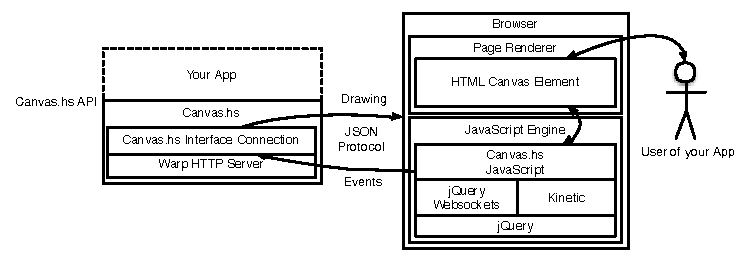
\includegraphics[keepaspectratio,width=\textwidth]{./images/architectuur_overzicht.pdf}
\caption{Overzicht  van Canvas.hs}
\label{fig:overzicht_canvas.hs}
\end{center}
\end{figure}

\subsubsection{Canvas.hs}
Canvas.hs is ontwikkeld met het oog op gebruiksgemak en eenvoud zonder de mogelijkheid tot uitbreiding en het toevoegen van geavanceerde functionaliteit onnodig te beperken.

\emph{Canvas.hs} is als library te installeren via \emph{Cabal}, de package manager voor Haskell programma's. In \autoref{sec:gebruikershandleiding} kan gelezen worden hoe de library gebruikt kan worden. Als een Haskell programma, via de aangeboden \emph{API}, de library aanroept zal een zeer lichte \emph{HTTP} en \emph{Websocket} server opgestart worden. Waarna de library een browser zal opstarten. Deze browser laadt de \emph{JavaScript} code van de library en toont vervolgens een \emph{HTML5 canvas} waar op getekend kan worden door het Haskell programma dat gebruik maakt van Canvas.hs. In \autoref{hoofdstuk:ontwerp} wordt het ontwerp van Canvas.hs beschreven.

De ontwikkelde library is uitgebreid getest. Dit geldt zowel voor de geschreven Haskell code als de JavaScript code. In \autoref{hoofdstuk:resultaten} kan hier meer over gelezen worden.

\subsubsection{Organisatie}
Bij de ontwikkeling van Canvas.hs is er gewerkt volgens eens vooraf vastgestelde afspraken. Daarnaast is er tooling toegepast om de samewerking tussen ontwikkelaars te stroomlijnen. \autoref{hoofdstuk:organisatie} beschrijft hoe dit alles is ingericht. Verder beschrijft \autoref{hoofdstuk:evaluatie}  hoe de afspraken en tools uiteindelijk zijn toegepast.

\subsubsection{Uitbreidingen}
Er zijn aanbevelingen voor de verdere verbetering van Canvas.hs. Hier wordt op in gegaan in \autoref{hoofdstuk:evaluatie} en \autoref{hoofdstuk:conclusie}. Verder is Canvas.hs opgezet zodat deze gemakkelijk is uit te breiden. In de \fullref{sec:uitbreiden} is te lezen hoe dit gedaan kan worden.


